\epigraph{``Since Newton, mankind has come to realise that the law of physics are always expressed in the language of differential equations"}{Steven Strogatz}

\section{RNN}
\subsection{Introduction}
Weather forecasting has traditionally been done by physical models of the atmosphere, which are unstable to perturbations, and thus are inaccurate for large periods of time\cite{why_rnn}. Since machine learning techniques are more sensitive to perturbations, it would be logical to combine a neural network with a physical model. Weather forecasting is a sequential data problem, therefore, a recurrent neural network is the most suitable option for this task. 

\begin{definition}
A recurrent neural network is a class of artificial neural networks where connections between nodes form a directed graph along a temporal sequence.
\end{definition}

Before, we delve into the specific example of using a recurrent neural network to predict the future state of the atmosphere, it is necessary to review what a recurrent neural network is. Recurrent Neural Networks (RNNs) are neural networks that are used in situations where data is presented in a sequence. For example, let's say you want to predict the future position of a fast-moving ball. Without information on the previous position of the ball, it is only possible to make an inaccurate guess. If you had, however, a large number of snapshots of the previous position, you are then able to predict the future position of the ball with some certainty. RNNs excel at modelling sequential data such as this. This is due to sequential memory.

In order to intuitively understand sequential memory, the prime example would be the alphabet. While it is easy to say the alphabet from A-Z, it is much harder to go from Z-A. There is a logical reason why this is difficult. As a child, you learn the alphabet in a sequence. Sequential memory is a mechanism that makes it easier for your brain to recognise sequence patterns.

In a traditional neural network, there is an input layer, hidden layer, and an output layer. In a recurrent neural network, a loop is added to pass information forward as seen in the diagram below (provided by Towards Data Science)\cite{intro_rnn}:

\begin{figure}[H]
    \centering
    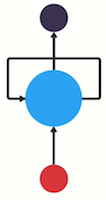
\includegraphics[width=.2\linewidth]{Images/rnn.png}
    \caption{Visualisation of a Recurrent Neural Network}
\end{figure}

The information that is forwarded is the hidden layer, which is a representation of previous inputs. How this works in practise is that you initialise your network layers and the initial hidden state. The shape and dimension of the hidden state will be dependent on the shape and dimension of your recurrent neural network. Then you loop through your inputs, pass the relevant parameter and hidden state into the RNN. The RNN returns the output and a modified hidden state. Last you pass the output of the hidden state to the output layer of the model, and it returns a prediction. 

There is, however, a major problem known as short-term memory. Short-term memory is caused by something known as the vanishing gradient problem, which is also prevalent in other neural network architectures. As the RNN processes more steps, it has troubles retaining information from previous steps. Short-Term memory and the vanishing gradient is due to the nature of back-propagation. This can be comprehended through understanding how a neural network is trained\cite{intro_rnn}.

\begin{definition}
Back-propagation is an algorithm used to train and optimise neural networks.
\end{definition}

To train a recurrent neural network, you use an application of back-propagation called back-propagation through time. Training a neural network has three major steps. First, the relevant data vector is normalised between 0 and 1, the vector is fed into the RNN, and it goes through an activation function. The activation function utilised in the software is the rectified linear activation function\cite{lstm_rnn}. 

\begin{definition}
The rectified linear activation function is a piece-wise linear function that will output the input directly if is positive, otherwise, it will output zero.
\end{definition}

The function is linear for values greater than zero, meaning it has a lot of the desirable properties of a linear activation function when training a neural network using back-propagation. Yet, it is a nonlinear function as negative values are always output as zero. As a result, the rectified function is linear for half of the input domain and nonlinear for the other half, it is referred to as a piece-wise linear function\cite{relu}. This nonlinear element is extremely important if the system has a nonlinear component, for example in predicting the evolution of the future state of the atmosphere.

\begin{figure}[H]
    \centering
    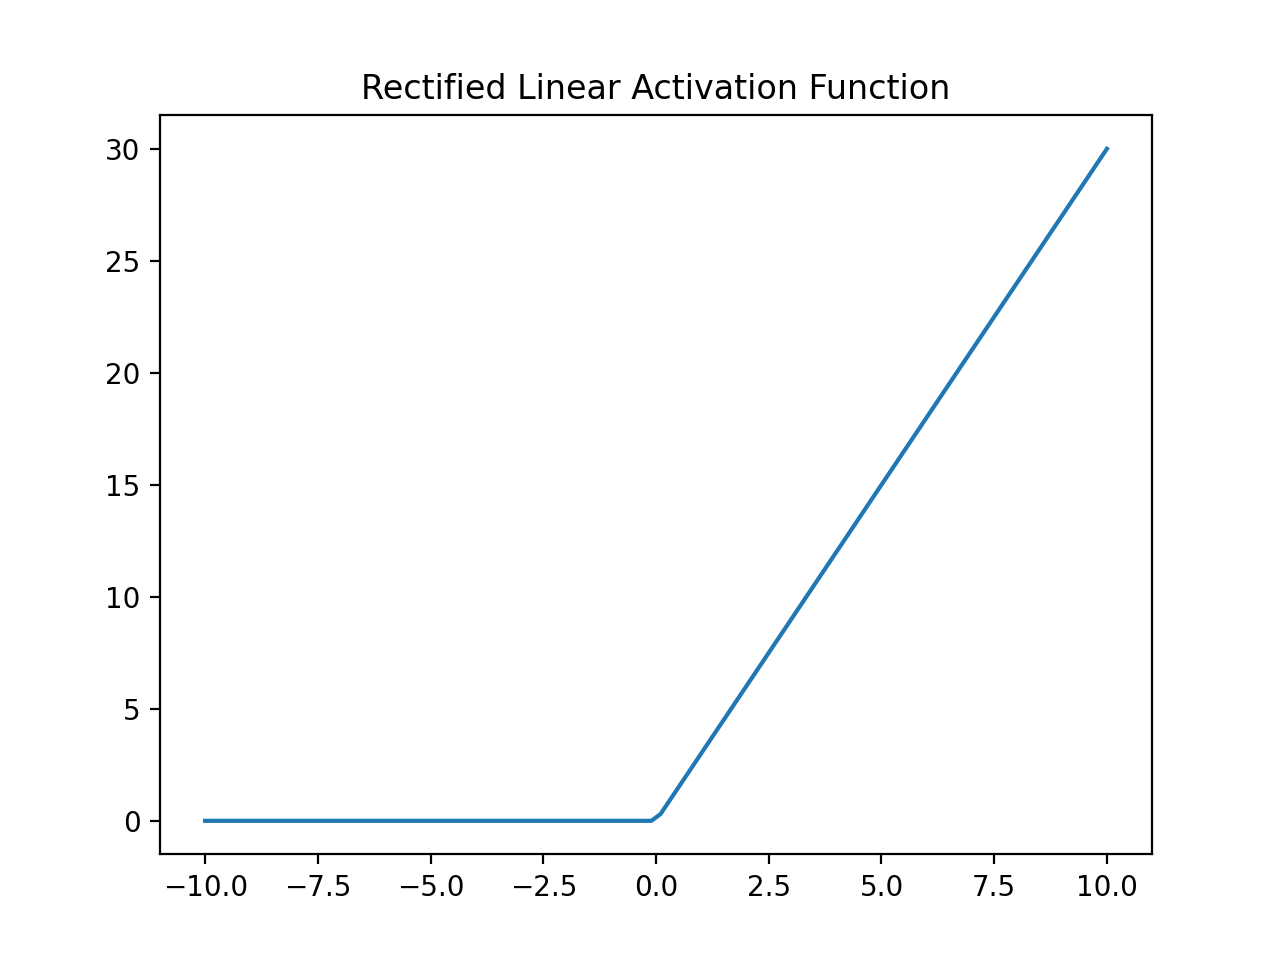
\includegraphics[width=.65\linewidth]{Images/relu.png}
    \caption{Sketch of the Rectified Linear Activation Function}
\end{figure}

Second, it outputs the results. Third, it compares the prediction to the observed state using a loss function.

\begin{definition}
A loss function outputs an error value which is an estimate of how poorly the network is performing.
\end{definition}

The lost function that will be utilised in the software will be the function for mean squared error. The reason for choosing this particular function is that it heavily penalises large errors, as it squares the difference between the predicted and actual value. A large error in a weather forecast is highly undesirable, hence, the use of this function. The function is represented below:

\begin{equation}
    MSE = \frac{1}{n}\sum_{i=1}^n(Y_i-\hat{Y_i})^2
\end{equation}

If  a vector of $n$ predictions is generated from a sample of $n$ data points on all variables, and $Y$ is the vector of observed values of the variable being predicted, with $\hat{Y_i}$ being the predicted values.

\begin{definition}
Mean squared error is the average squared difference between the estimated values and the actual value.
\end{definition}

Returning to the training of the RNN, it uses that error value from the loss function to do back propagation which calculates the gradients for each time step in the network. The gradient is the value used to adjust the networks internal weights, allowing the network to learn. The bigger the gradient, the bigger the adjustments and vice versa. Here is where the problem lies. When doing back propagation, the gradient of the current time step is calculated with respect to the effects of the gradients, in the time step before it. So if the adjustments to the time step before it is small, then adjustments to the current time step will be even smaller.  The gradient values will exponentially shrink as it propagates through each time step. That causes gradients to exponentially shrink as it back propagates down. The earlier layers fail to do any learning as the internal weights are barely being adjusted due to extremely small gradients.

Because of vanishing gradients, the RNN doesn’t learn the long-range dependencies across time steps. So not being able to learn on earlier time steps causes the network to have a short-term memory. In order to combat this, a long short-term memory is used\cite{intro_rnn}.

\subsection{LSTM}
LSTM's were created as a solution to the short-term memory problem. They have internal mechanisms called gates that can regulate the flow of information. These gates can learn which data in a sequence is important to keep or throw away. By doing that, it can pass relevant information down the long chain of sequences to make predictions. For example, if you were interested in buying a particular product, you might read a review in order to determine if the purchase of the product is a good decision. When you read a review, your brain subconsciously only remembers important keywords. You pick up words like ``amazing", ``superb", or ``awful", you don't remember words such as "the", "as", or "because". This is what an LSTM does, it learns to keep only the relevant information to make predictions.

An LSTM has a similar control flow as a recurrent neural network. It processes data passing on information as it propagates forward. The differences are the operations within the LSTM’s cells. The core concept of LSTM’s are the cell state, and it’s various gates. The cell state is the method by which information is transferred down the sequence chain. The cell state, in theory, can carry relevant information throughout the processing of the sequence. So even information from the earlier time steps can make its way to later time steps, reducing the effects of short-term memory. As the cell state goes on its journey, information gets added or removed to the cell state via gates\cite{lstm_rnn}.

\begin{definition}
A gate is an electric circuit with an output which depends on the combination of several inputs.
\end{definition}

Gates contain the sigmoid activation function. The sigmoid activation function squishes values between 0 and 1. That is helpful to update or forget data because any number getting multiplied by 0 is 0, causing values to disappears or be ``forgotten". Any number multiplied by 1 is the same value therefore that value stays the same or is ``kept".

\begin{figure}[H]
    \centering
    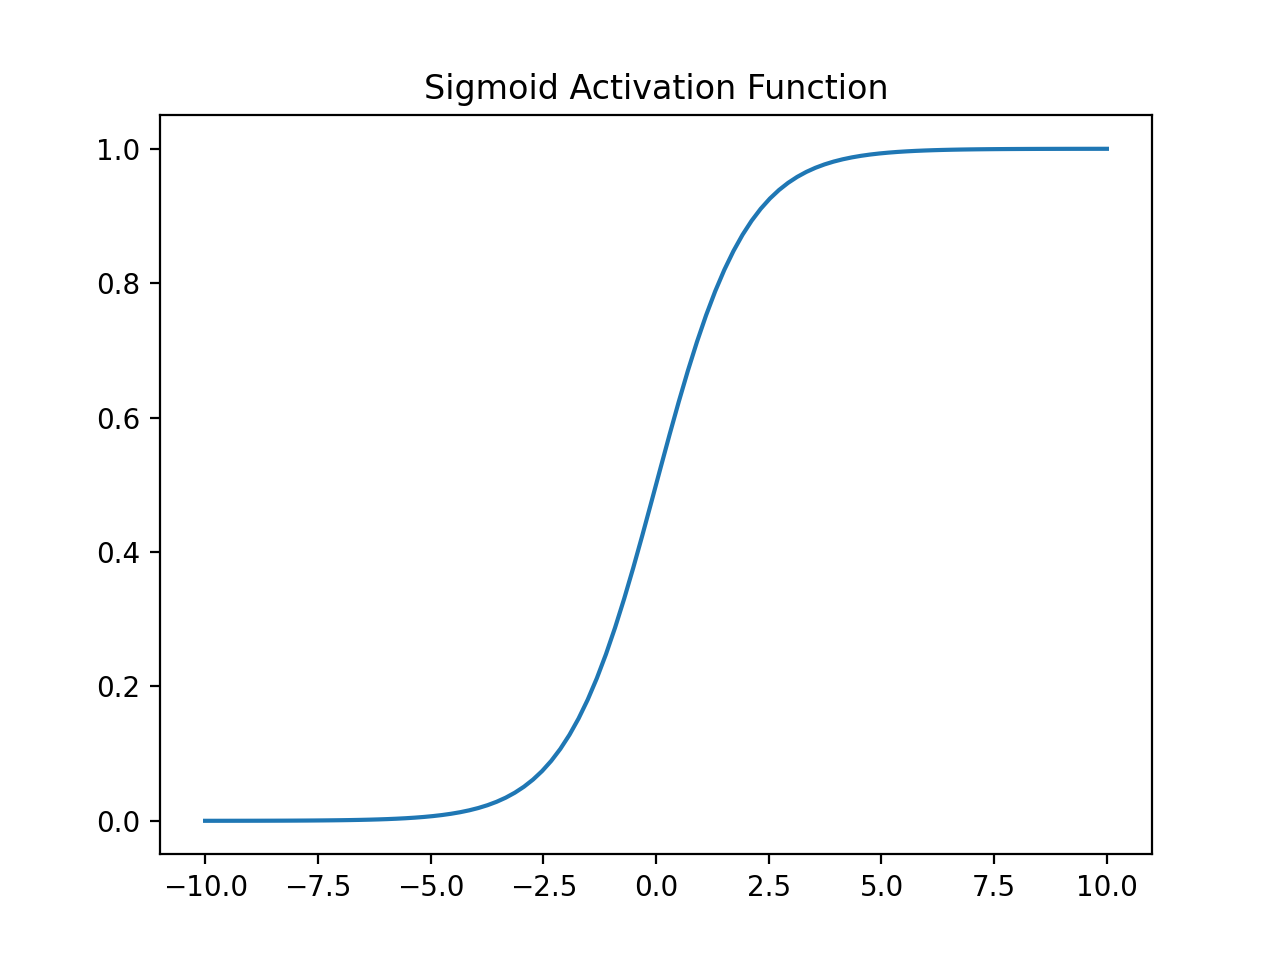
\includegraphics[width=.65\linewidth]{Images/sigmoid.png}
    \caption{Sketch of the Sigmoid Activation Function}
\end{figure}

There are three types of gates utilised within a neural network: a forget gate, an input gate, and an output gate. A forget gate decides what information should be thrown away or kept. Information from the previous hidden state and information from the current input is passed through the sigmoid function. An input gate is where the previous hidden state and current input are passed into a sigmoid function. The output gate decides what the next hidden state should be. The hidden state is also used for predictions. First, we pass the previous hidden state and the current input into a sigmoid function. Then we pass the newly modified cell state to the rectified linear activation function. We multiply the rectified linear activation function output with the sigmoid output to decide what information the hidden state should carry. The output is the hidden state. The new cell state and the new hidden state is then carried over to the next time step\cite{lstm_rnn}.

\subsection{Convolutional LSTM Network}
The formulation of a numerical weather prediction model is a spatiotemporal sequence forecasting problem that can be solved under a general sequence-to-sequence learning framework. 

\begin{definition}
A spatiotemporal sequence is a sequence that contains both spatial and temporal information.
\end{definition}

In order to better model the spatiotemporal relationships, this project will utilise ConvLSTM layers; which was proposed by Xingjian Shi et. al\cite{convlstm}. This spatiotemporal sequence forecasting problem is different from the one-step time series forecasting problem because the prediction target of the problem is a sequence which contains both spatial and temporal structures. Although a LSTM layer has proven powerful for handling temporal correlation, it contains too much redundancy for spatial data. To address this problem, this project will use a ConvLSTM layer which has convolutional structures in both the input-to-state and state-to-state transitions\cite{convlstm}.

The major drawback of LSTMs is in the handling spatiotemporal data due to its usage of full connections in input-to-state and state-to-state transitions in which no spatial information is encoded. To overcome this problem, a distinguishing feature of a ConvLSTM cell is that all the inputs and gates of the ConvLSTM layer are 3D tensors whose last two dimensions are spatial dimensions. To get a better picture of the inputs and states, we may imagine them as vectors standing on a spatial grid. The ConvLSTM determines the future state of a certain cell in the grid by the inputs and past states of its local neighbour. This can easily be achieved by using a convolution operator in the state-to-state and input-to-state transitions\cite{convlstm}. This is what the ConvLSTM layer does.

\begin{figure}[H]
    \centering
    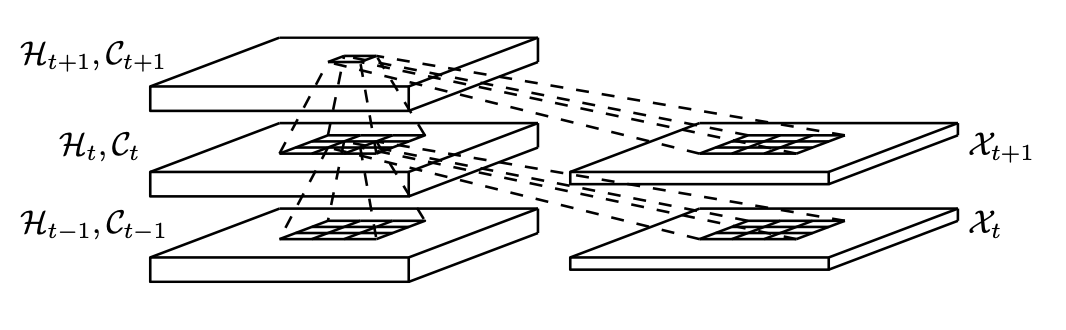
\includegraphics[width=.8\linewidth]{Images/convlstm.png}
    \caption{The architecture of a ConvLSTM cell.}
\end{figure}

\section{Dataset}
\subsection{ERA5 Atmospheric Reanalysis Dataset}\label{era5_dataset}
ERA5 provides hourly estimates of a large number of atmospheric, land and oceanic climate variables. The data covers the Earth on a 30km grid and resolves the atmosphere using 137 levels from the surface up to a height of 80km. ERA5 includes information about uncertainties for all variables at reduced spatial and temporal resolutions. Quality-assured monthly updates of ERA5 are published within 3 months of real time. Preliminary daily updates of the dataset are available to users within 5 days of real time. ERA5 combines vast amounts of historical observations into global estimates using advanced modelling and data assimilation systems\cite{era5}.

The ERA5 reanalysis dataset was used for training, validating and testing the performance of the neural network architecture. Reanalysis datasets provide the best guess of the atmospheric state at any point in time by combining a forecast model with the available observations. The raw data is available hourly for 40 years from 1979 to 2019 on a $0.25^{\circ}$ latitude-longitude grid ($721 \times 1440$ grid points) with 37 vertical levels. Since this raw dataset is quite significant, it is necessary to regrid the dataset to a lower resolution and use a smaller fraction of the available dataset\cite{rasp2020weatherbench}.  The poles were excluded from the dataset in order to avoid a singularity, and the potential negative impact that could have on predictive ability of the neural network.

It was ultimately decided to use a spatial resolution of $1^{\circ}$ ($179 \times 360$ grid points) and a temporal resolution of 2 hours. The data is split into yearly NetCDF files for each variable. The entire dataset at $0.25^{\circ}$ resolution has a size of 400GB, before the dataset was interpolated to a grid of a lower resolution. The prognostic variables of interest are temperature and geopotential, and were chosen based on meteorological considerations. Geopotential, and temperature are prognostic state variables in most physical numerical weather prediction and climate models\cite{rasp2020weatherbench}. 

\subsection{Integrated Forecasting System}\label{ifs_section}
The Integrated Forecast System is a global numerical weather prediction system developed and maintained by the European Centre for Medium-Range Weather Forecasts organisation. The version of the IFS run at ECMWF is often referred to as the ``ECMWF" or the ``European model" in North America, to distinguish it from the American GFS. It comprises of a spectral atmospheric model with a terrain-following vertical coordinate system coupled to a 4D variational data assimilation system. In 1997 the IFS became the first operational forecasting system to use a 4D variational, data assimilation system

\begin{definition}
4D dimensional variational data assimilation system adjusts a short-range forecast, called the background, in space and time to bring it into closer agreement with meteorological observations.
\end{definition}

\begin{figure}[H]
    \centering
    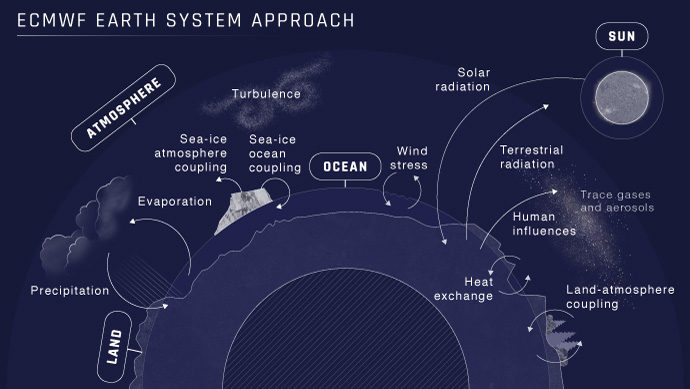
\includegraphics[width=.8\linewidth]{Images/ifs.jpg}
    \caption{ECMWF Integrated Forecast System}
\end{figure}

It is one of the predominant global medium-range models in general use worldwide; its most prominent rival in the 6–10 day medium range include the American Global Forecast System, the Canadian Global Environmental Multiscale Model and the UK Met Office Unified Model. For context, Met Éireann utilises the IFS for medium-range forecasts; however for short-range forecasts, Met Éireann uses its own HARMONIE-AROME NWP model. The operational configuration consists of $1000 \times 900$ grid points in the horizontal at 2.5km resolution, with 65 levels in the vertical. A 54-hour forecast is produced four times a day, at 00Z, 06Z, 12Z and 18Z\cite{harmonie_arome_nwp}. 

The IFS is the gold standard of medium-range numerical weather prediction. The current IFS deterministic forecast is computed on a cluster with 11,664 cores. One 10 day forecast at 10 km resolution takes around 1 hour of real time to compute\cite{rasp2020weatherbench}. The Integrated Forecasting System will be used as a comparison against the neural network.

To provide physical baselines more in line with the current resolution of the neural network, it was compared against the IFS model at two coarser horizontal resolutions, T42 (approximately $2.8^{\circ}$) with 62 vertical levels and T63 (approximately $1.9^{\circ}$) with 137 vertical levels. It must be noted that I personally did not generate such forecasts, or perform the analysis on said forecasts. It acquired the results from Weather Bench, a benchmark dataset for data-driven weather forecasting. According to said source; computationally, a single forecast takes 270 seconds for the T42 model and 503 seconds for the T64 model on a single XC40 node with 36 cores.

\section{Implementation}\label{implement_rnn}
Drawing from knowledge of current numerical weather prediction model frameworks, it may seem intuitive to train a machine learning model to produce the best possible single‐step forecast from a given atmospheric state. In practice, this can yield a model that performs well for short‐range forecasts but diverges from reality for longer range predictions. This is because there are no constraints on the CNN, physical or mathematical, that would prevent it from diverging from reality when its prediction fed back in as inputs no longer resemble an atmospheric state in the training data. In order to nudge the numerical weather prediction model toward learning to predict longer‐term weather and improve its long‐term stability, the model will be trained on multiple iterated predictive steps. 

Initially, the model inputs included two time steps and it is tasked with predicting two output time steps. This resulted in the first couple of time step predictions producing relatively decent result, however, it quickly diverged from reality after this point. Hence, it was necessary to increase both the time steps and the output time steps to six. This increased the overall numerical stability of the model. 

The dataset consists of three features: air temperature at a pressure surface of 850 hPa, geopotential at a pressure surface of 500 hPa, and air temperature at 2 metres above the surface. For a single day, there is twelve observations. The goal for this project will be to predict the relevant atmospheric parameter in 12 hours time given the last twelve hours of data. In order to make such predictions, it is necessary to create a window of the last 6 ($\frac{12}{2}$) observations to train the model\cite{time_series}. The neural network was trained on observational data from 2009 to 2015. The remainder of the dataset, 2016 to 2019, was preserved for validation, testing and benchmarking the neural network against physics-based models. The model was built using the open‐source Keras library for Python with Google's TensorFlow backend\cite{numerical_stability}.

\begin{minted}[mathescape,linenos,frame=lines]{python}
# Optimiser.
opt = Adam(lr=1e-3, decay=1e-5)
\end{minted}

Adam optimisation was chosen as the most appropriate optimiser for this particular model. This is a stochastic gradient descent method that is based on adaptive estimation of first-order and second-order moments. This method is computationally efficient, has little memory requirements, invariant to diagonal rescaling of gradients, and is well suited for problems that are large in terms of parameters.

\begin{minted}[mathescape,linenos,frame=lines]{python}
# First layer of model.
model.add(
    ConvLSTM2D(
        filters=64, 
        kernel_size=(7, 7),
        input_shape=(6, 179, 360, 3), 
        padding='same', 
        return_sequences=True, 
        activation='tanh', 
        recurrent_activation='hard_sigmoid',
        kernel_initializer='glorot_uniform', 
        unit_forget_bias=True, 
        dropout=0.3, 
        recurrent_dropout=0.3, 
        go_backwards=True
    )
)
\end{minted}

The above code is the first layer of the model. The activation functions utilised in this layer are predefined within Tensorflow, and have been described at great length previously. The model consists of four ConvLSTM layers in total, with similar parameters as the aforementioned layer with a few variations.

\begin{minted}[mathescape,linenos,frame=lines]{python}
# Batch normalisation.
model.add(BatchNormalization())
\end{minted}

A consistent challenge in machine learning is that the model is updated layer-by-layer backward from the output to the input using an estimate of error that assumes the weights in the layers prior to the current layer are fixed. Because all layers are changed during an update, the update procedure is forever chasing a moving target. A batch normalisation layer occurs after each ConvLSTM layer to resolve this problem.  

\begin{definition}
Batch normalization is a technique to help coordinate the update of multiple layers in the model.
\end{definition}

It does this by scaling the output of the layer, specifically by standardising the activation of each input variable per mini-batch, such as the activation of a node from the previous layer. Standardising the activation of the prior layer means that assumptions the subsequent layer makes about the spread and distribution of inputs during the weight update will not change. This has the effect of stabilising and speeding-up the training process of neural networks\cite{batch_normalization}.

\begin{minted}[mathescape,linenos,frame=lines]{python}
# Dropout.
model.add(Dropout(0.1))
\end{minted}

Each batch normalisation layer is then followed by a dropout. Dropout is a regularisation method that approximates training a large number of neural networks with different architectures in parallel. During training, some number of layer outputs are randomly ignored or “dropped out.” This has the effect of making the layer look-like and be treated-like a layer with a different number of nodes and connectivity to the prior layer. In effect, each update to a layer during training is performed with a different “view” of the configured layer. Dropout has the effect of making the training process noisy, forcing nodes within a layer to probabilistically take on more or less responsibility for the inputs. This conceptualisation suggests that perhaps dropout breaks-up situations where network layers co-adapt to correct mistakes from prior layers, in turn making the model more robust\cite{dropout}.

\begin{minted}[mathescape,linenos,frame=lines]{python}
# Add dense layer.
model.add(Dense(3))
\end{minted}

Following the final ConvLSTM layer, a dense layer is implemented. The dense layer is a neural network layer that is connected deeply, which means each neuron in the dense layer receives input from all neurons of its previous layer\cite{dense}. In our case, it results in the model outputting the expected shape by reducing the filters down to the three previously mentioned features. The code for the model in its entirety can be found in appendix \ref{model_code}. 
